\section{Alit Fajar Kurniawan}
{\Large \textbf{Pemahaman Teori}}
\subsection{No. 1}
Apa itu fungsi device manager di windows dan folder /dev di linux?

	\hfill \break
	Device manager adalah perangkat lunak untuk menampilkan seluruh perangkat keras yang diinisialisasi atau sudah terhubung dengan sistem operasi Windows. Perangkat keras tersebut bisa berupa harddisk, kartu VGA, sound, keyboard, perangkat USB dan lain-lainnya. fungsi lain dari device manager yaitu, Menunjukkan status mengenai suatu perangkat keras,
	Mengelola driver perangkat keras, Menonaktifkan dan mengaktifkan perangkat keras, Menunjukkan informasi detail mengenai suatu perangkat keras, Mengidentifikasi konflik antar perangkat keras, dan Memberitahukan terjadinya masalah pada perangkat keras.

	\hfill \break
	Folder /dev merupakan representasi dari drive yang terhubung ke sistem operasi Linux dan oleh sistem dianggap sebagai file-file direktori. Biasanya sering ditampilkan direktori seperti /dev/sda1 yang mewakili Drive SATA pertama dalam sistem.

\subsection{No. 2}
Jelaskan langkah-langkah instalasi driver dari arduino!

	\hfill \break
	Berikut ini adalah langkah-langkah instalasi driver dari Arduino UNO di Windows:

	\begin{enumerate}
		\item Pertama pastikan Arduino IDE telah terinstall.
		\item Lalu hubungkan port USB Arduino Uno ke port USB PC.
		\item Kemudian PC anda akan mendeteksi perangkat baru yang terpasang dan akan muncul pop seperti ini.
		\item Karena Arduino Uno baru pertama kali terpasang, maka akan muncul pop up error seperti ini.
		\item Buka ''Start'' lalu cari Device Manager, kemudian klik ''Device Manager''.
		\item Setelah Device Manager terbuka, silahkan cari ''Unknown Device'' yang berada di Other Device.
		\item Kemudian klik kanan pada ''Unknown Device'', lalu pilih ''Update Driver Software''.
		\item Setelah itu muncul window baru, lalu pilih ''Browse my computer for driver software''.
		\item Lalu cari folder yang terinstall Arduino IDE dengan mengklik browse. Kemudian klik ''Next''.
		\item Windows akan mencari dan menginstall driver yang berada pada folder tersebut.
		\item Setelah itu akan muncul window, lalu klik ''Install''.
		\item Jika berhasil terinstal maka akan muncul window seperti ini.
	\end{enumerate}

\subsection{No. 3}
	\begin{itemize}
		\item Membaca Baudrate dari Komputer
			\begin{enumerate}
				\item Pertama buka ''Start''. Cari ''Device Manager'', lalu klik.
				\item Kemudian pilih ''Ports (COM \& LPT)''.
				\item Klik dua kali pada COM yang terhubung.
				\item Pilih tab ''Port Settings'', lalu lihat di ''Bit per second''.
			\end{enumerate}
		\item Membaca Port dari Komputer
			\begin{enumerate}
				\item Pertama buka ''Start''. Cari ''Device Manager'', lalu klik.
				\item Kemudian pilih ''Ports (COM \& LPT)''.
				\item Port dari Arduino telah terbaca oleh PC.
			\end{enumerate}
	\end{itemize}
	
\subsection{No. 4}
	Jelaskan sejarah library pyserial!

	\hfill \break
	PySerial adalah paket Python yang menfasilitasi komunikasi serial antara PC dengan perangkat keras eksternal. PySerial menyediakan antarmuka untuk berkomunikasi melalui protokol komunikasi serial. Komunikasi serial adalah salah satu protokol komunikasi komputer tertua. Protokol komunikasi serial mendahului spesifikasi USB yang digunakan oleh komputer dan perangkat keras lain seperti mouse, keyboard, dan webcam. USB adalah singkatan dari Universal Serial Bus. USB dan dibangun di atas dan memperluas antarmuka komunikasi serial asli.

\subsection{No. 5}
	Jelaskan fungsi-fungsi apa saja yang dipakai dari library pyserial!

	\hfill \break
	Fungsi-fungsi yang dipakai dari library PySerial, yaitu:
	\begin{enumerate}
		\item Serial - fungsi ini untuk membuka port serial.
		\item write(data) - fungsi ini menulis data lewat port serial.
		\item readline - fungsi ini membaca sebuah string dari port serial.
		\item read(size) - fungsi ini untuk membaca jumlah byte dari port serial.
		\item close - fungsi ini untuk menutup port serial.
	\end{enumerate}

\subsection{No. 6}
	Jelaskan kenapa butuh perulangan dan tidak butuh perulangan dalam membaca serial!

	\hfill \break
	Pada saat membaca serial di Arduino diperlukan perulangan agar bisa membaca data secara berulang kali sehingga data yang muncul banyak. Sedangkan apabila tidak membutuhkan perulangan maka Arduino hanya akan membaca data sekali saja.

\subsection{No. 7}
	Jelaskan bagaimana cara membuat fungsi yang mengunakan pyserial!

	\lstinputlisting[caption = Fungsi yang menggunakan pyserial., firstline=1, lastline=13]{src/chapter5/teori/1174057.py}

	\subsection{Cek Plagiat}
	\begin{figure}[H]
		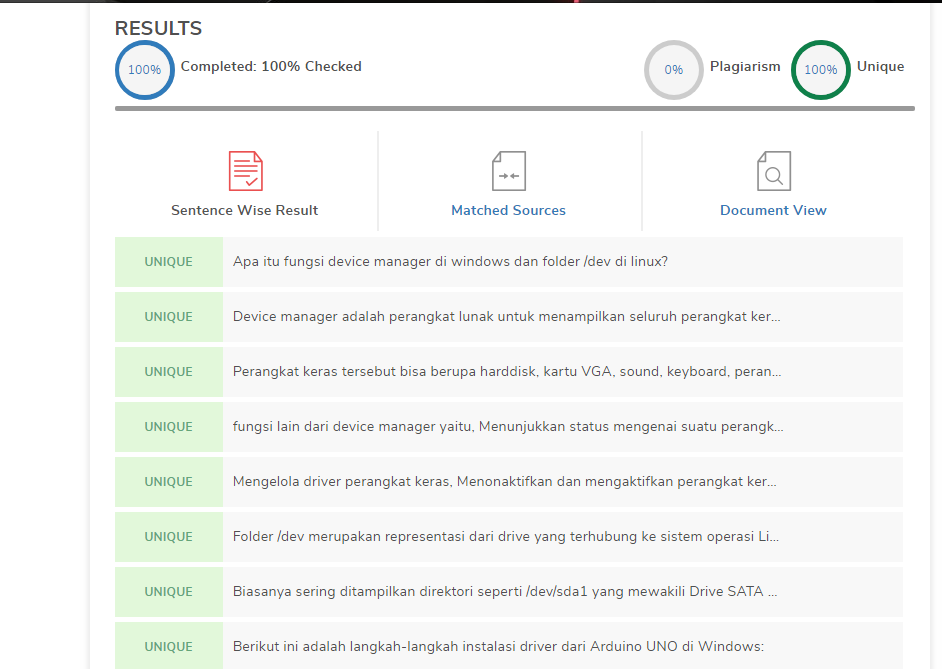
\includegraphics[width=10cm]{figures/chapter5/1174057/teori/plagiarisme.png}
		\centering
		\caption{Hasil cek plagiat}
	\end{figure}
	
	
\section{Muhammad Iqbal Panggabean}
{\Large \textbf{Pemahaman Teori}}
\subsection{Pertanyaan No.. 1}
Apa itu fungsi device manager di windows dan folder /dev di linux?

\hfill \break
Fungsi device manager antara lain :
\begin{enumerate}
	\item Mengidentifikasi konflik antar perangkat keras.
	\item Menunjukkan informasi detil suatu hardware.
	\item Disable dan Enable hardware.
	\item Mengelola driver hardware.
	\item Menunjukkan status suatu hardware.
\end{enumerate}

\hfill \break
Folder /dev berisi file device, baik device blok maupun device karakter. Di dalamnya setodaknya ada file biner yang beernama MAKEDEV untuk membuat device secara manual.

\subsection{Pertanyaan No. 2}
Jelaskan langkah-langkah instalasi driver dari arduino!

\hfill \break
Berikut ini adalah langkah-langkah instalasi driver dari Arduino UNO di Windows:

\begin{enumerate}
	\item Hubungkan sistem minimun Arduino Uno ke komputer dengan kabel USB type B (kabel Printer).
	\item Lalu pada bagian kanan didesktop PC anda, akan muncul popup “Installing device driver software”.
	\item SIstem operasi Windows tidak menyediakan driver untuk Arduino Uno.
	\item Buka Device Manager, caranya pada bagian Search Program and Files lalu ketikkan “device manager” (tanpa tanda petik). Kemudian bagian Control Panel akan muncul halaman Device Manager, selanjutnya klik untuk menjalankan.
	\item Cari yang bernama Unknown device yang berada pada bagian Other device, biasanya ada tanda seru berwarna kuning, itu disebabkan karena penginstallan tidak berjalan dengan sempurna.
	\item Klik kanan pada “Unknown device” kemudian pilih Update Driver Software.
	\item Pilih Browse my computer for driver software.
	\item Arahkan lokasi folder ke folder ..arduino-1.0.5 drivers. Pastikan check-box lalu centang include subfolders. Klik Next untuk melanjutkan instalasi driver.
	\item Kemudian lanjutkan dengan mengklik Install pada tampilan Windows Security.
	\item Jika instalasi driver berhasil maka akan muncul Windows has successfully updated your driver software.
	\item Perhatikan dan ingat nama COM Arduino Uno, karena nama COM ini yang akan digunakan untuk meng-upload program nantinya.
\end{enumerate}

\subsection{Pertanyaan No. 3}
Jelaskan bagaimana cara membaca baudrate dan port dari komputer yang sudah terinstall driver!

\hfill \break
\textbf{Membaca Port dari Komputer}

\begin{enumerate}
	\item Hubungkan modul TX-RX serial dengan komputer melalui serial port menggunakan DB9 cable extension.
	\item Buka Hyper Terminal dengan menekan start kemudian All progams lalu Accessories kemudian Communications lalu Hyper Terminal.
	\item Ketik nama untuk Connection Description, misal coba, kemudian tekan OK.
	\item Pada Connect to, pilihlah COM port yang dipakai di Connect using, kemudian tekan OK.
	\item Masukkan nilai-nilai port settingnya, sesuai dengan DCE-nya. Kemudian tekan OK.
\end{enumerate}



\subsection{Pertanyaan No. 4}
Jelaskan sejarah library pyserial!

\hfill \break
PySerial adalah library/modul Python siap-pakai dan gratis yang dibuat untuk memudahkan kita dalam membuat program komunikasi data serial RS232 dalam bahasa Python.
Jika modul USB-2REL dapat kita kontrol dengan mudah menggunakan Python dan PyUSB (lihat pembahasannya di sini dan di sini), maka modul SER-2REL juga dapat kita kontrol dengan mudah menggunakan Python dengan bantuan modul PySerial.

\subsection{Pertanyaan No. 5}
Jelaskan fungsi-fungsi apa saja yang dipakai dari library pyserial!

\hfill \break
Fungsi-fungsi yang dipakai dari library PySerial, yaitu:
\begin{enumerate}
	\item Serial - fungsi ini untuk membuka port serial.
	\item write(data) - fungsi ini menulis data lewat port 
	\item serial.close() - fungsi ini untuk menutup port serial.
	\item readline() - fungsi ini membaca sebuah string dari port serial.
	\item read(size) - fungsi ini untuk membaca jumlah byte dari port serial.
\end{enumerate}

\subsection{Pertanyaan No. 6}
Jelaskan kenapa butuh perulangan dan tidak butuh perulangan dalam membaca serial!

\hfill \break
Pada saat membaca serial di Arduino diperlukan perulangan agar bisa membaca data secara berulang kali sehingga data yang muncul banyak. Sedangkan apabila tidak membutuhkan perulangan maka Arduino hanya akan membaca data sekali saja.

\subsection{Pertanyaan No. 7}
Jelaskan bagaimana cara membuat fungsi yang mengunakan pyserial!

\hfill \break
Fungsi yang berada pada Python, dibuat dengan nama kata kunci def kemudian diikuti dengan nama fungsinya pada pyhton.
Seperti halnya dengan blok kode yang lain, kita juga harus memberikan identasi untuk menuliskan isi fungsi.

\subsection{Cek Plagiat}
\begin{figure}[H]
	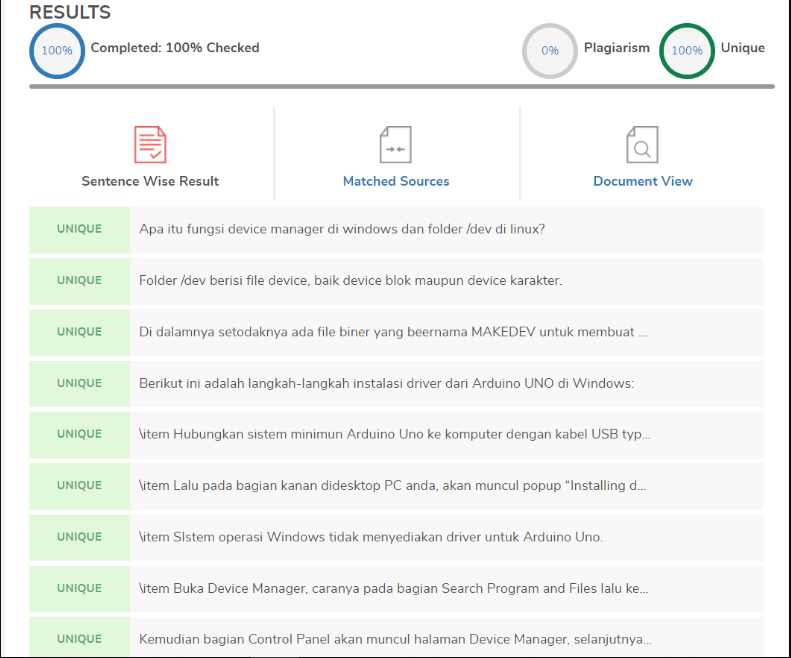
\includegraphics[width=10cm]{figures/5/1174063/Teori/plagiatgabe.png}
	\centering
	\caption{Hasil cek plagiat.}
\end{figure}